\documentclass[11pt, a4paper]{article}
\usepackage[T1]{fontenc} 
\usepackage[utf8]{inputenc}
\usepackage[czech]{babel}
\usepackage[left=2cm, top=1cm, bottom=1.5cm, text={17cm, 24cm}]{geometry}
\usepackage{graphicx}
\usepackage{titlesec}
\usepackage{enumitem}
\usepackage{array,tabularx}
\usepackage{times}
\usepackage{float}
\usepackage{minted}

\titleformat*{\section}{\LARGE\bfseries}

\begin{document}
\pagenumbering{arabic}
\setcounter{page}{1}

\begin{center}
   
{\textbf{\Huge IZV - Analýza nehod}}

\vspace{0.5cm}

{\textbf{\Huge Nehody, součástí kterých byla Policie ČR}}

    
\end{center}
\begin{LARGE}

{\LARGE Autor: Karel Norek, xnorek01 \hfill \today}
\end{LARGE}

\vspace{1cm}

\LARGE
\noindent
Na českých silnicích dochází každoročně k několika desítkám tisíc nehod. V této práci se však zaměříme na ty nehody, které zahrnují služební auta Policie ČR. Tímto zahrnutím se myslí jakékoliv figurování služebního auta Policie ČR při autonehodě, bez ohledu na to, je-li nehoda zaviněna jiným řidičem, nebo přímo policií. Následné řešení nehod Policií ČR se sem však nezahrnuje.

\section{Nehody podle krajů}
Nejdříve se podívame na situaci v jednotlivých krajích.

\begin{figure}[ht]
    \centering
    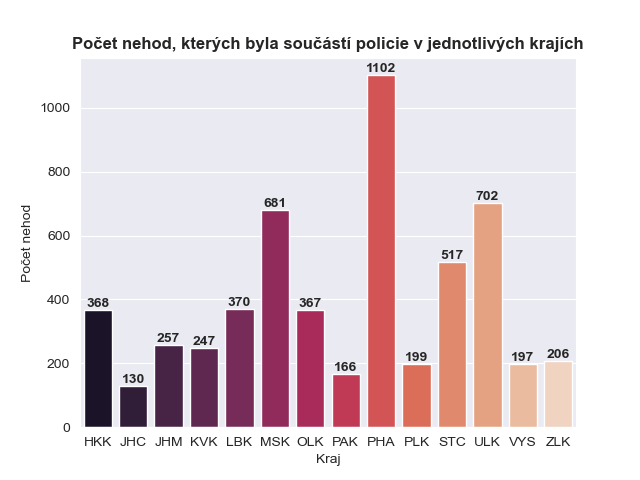
\includegraphics[scale=0.8]{police.png}
    \caption{Nehody v jednotlivých krajích}
    \label{fig:graph}
\end{figure}

Průměrný počet nehod v krajích je 364. V grafu lze vidět, že kraj Praha má více než trojnásobek pruměru. Z toho lze usoudit, že nehody Policie jsou nejvíce ve městech. V letech 2016-2021 je nejvyšší počet nehod v kraji Praha a to 1102 nehod. Nejmeněší počet nehod má Jihočeský kraj se 130 nehodama. Celkový počet nehod pak číní 5509.

\section{Nehody podle typu komunikace}
Dále se podívame na nehody podle určitého typu komunikace.

\def\arraystretch{1.5}
\begin{table}[ht]
\scalebox{0.85}{
\begin{tabular}{|l|r|r|r|r|r|r|}
\toprule \hline
Druh komunikace &  Dvoupruhová &  Rychlostní komunikace &  Třípruhová &  Vícepruhová &  Čtyřpruhová &  Žádná z uvedených \\
Rok  &              &                        &             &              &              &                    \\
\midrule \hline
2016 &        637.0 &                    4.0 &        53.0 &         11.0 &         44.0 &              203.0 \\ \hline
2017 &        695.0 &                    2.0 &        48.0 &         24.0 &         38.0 &              229.0 \\ \hline
2018 &        630.0 &                    5.0 &        38.0 &         22.0 &         27.0 &              222.0 \\ \hline
2019 &        614.0 &                    3.0 &        53.0 &         18.0 &         52.0 &              195.0 \\ \hline
2020 &        671.0 &                    0.0 &        57.0 &         19.0 &         41.0 &              186.0 \\ \hline
2021 &        457.0 &                    1.0 &        19.0 &         12.0 &         36.0 &              143.0 \\ \hline
\bottomrule
\end{tabular}
}
\caption{Počet nehod policie ČR v jednotlivých letech na ruzných komunikacích}
\label{fig:table}
\end{table}

Z dat lze vidět, že se počet nehod na určitých druzích silnic přiliž nemění, až na rok 2021, který ještě není kompletní. 

Mužeme vidět, že nejvíce nehod je na dvoupruhových silnicích a nejméně na rychlostních silnicích. Pomocí těchto dat lze usoudit, kde se auta Policie pohybují také nejvíce a kde nejméně. 

\end{document}